% ----------------------------------------------------------
% Apêndices v2
% ----------------------------------------------------------
\begin{apendicesenv}

% ----------------------------------------------------------
\chapter{Quadro Síntese das Abordagens sobre (I)Racionalidade Humana e Política}
% ----------------------------------------------------------
\label{apendice:quadro_iracionalidade}

{\renewcommand{\LTcaptype}{quadro}
 \captionsetup{type=quadro}
 \begin{longtable}{p{0.15\textwidth} p{0.23\textwidth} p{0.34\textwidth} p{0.20\textwidth}}
 \caption{Quadro Síntese – (I)Racionalidade Humana e Política: Principais Abordagens}
 \\

 \toprule
 \textbf{Autor/Obra (Ano)} & \textbf{Tópico/Conceito Central} & \textbf{Principais Contribuições e Evidências} & \textbf{Relação com o TCC} \\
 \midrule
 \endfirsthead

 \multicolumn{4}{r}{\small\textbf{Quadro \thequadro\ (continuação)}}\\
 \toprule
 \textbf{Autor/Obra (Ano)} & \textbf{Tópico/Conceito Central} & \textbf{Principais Contribuições e Evidências} & \textbf{Relação com o TCC} \\
 \midrule
 \endhead

 \midrule
 \multicolumn{4}{r}{\small\itshape Continua na próxima página}\\
 \endfoot

 \bottomrule
 \multicolumn{4}{l}{\footnotesize Fonte: elaboração própria.}
 \endlastfoot

 Adam Smith (1759; 1776) & Moralidade e racionalidade econômica & Integra interesse próprio e normas morais; reconhece limites do modelo racional estrito. & Critica o \textit{homo economicus} e destaca a ética na decisão pública. \\
 Herbert Simon (1955) & Racionalidade Limitada & Mostra que decisões são feitas com informação e tempo limitados; ``satisficing''. & Base para analisar limites cognitivos em escolhas políticas. \\
 Kahneman \& Tversky (1974, 2011) & Heurísticas e Vieses Cognitivos & Representatividade, ancoragem etc. & Explica previsibilidade dos desvios do eleitor médio. \\
 Anthony Downs (1957) & Ignorância Racional & Custo de informar-se > benefício do voto. & Fundamenta debate sobre baixa informação e democracia. \\
 Bryan Caplan (2007) & Irracionalidade Racional & Crenças falsas por motivações emocionais. & Viés sistemático com impacto em políticas. \\
 Hayek (1945) & Limitação do conhecimento & Conhecimento disperso; centralização inviável. & Crítica à ilusão de controle racional. \\
 Sapienza \& Zingales (2013) & Economistas vs.\ americanos médios & Formação e ideologia operam como duo; ambos predizem divergências. & Moldura analítica central deste TCC. \\
 Fuller \& Geide-Stevenson (2014) & Consenso entre economistas & Amplo consenso em livre-comércio, produtividade, livre-mercado. & Padrão de referência para direção esperada dos coeficientes de \texttt{econ}. \\
 Gelman \& Carlin (2014) & Retrodesign (Tipo S e Tipo M) & Erros de sinal e magnitude em estudos com baixo poder. & Interpretação do resultado nulo BH com $n_{\texttt{econ}} = 17$. \\
 Bhagwati, Sowell, Bastiat & Viés antimercado/antiestrangeiro & Protecionismo recorrente e argumentos populares. & Vieses e políticas populistas. \\
 Nyhan, Kahan, Sunstein, Rossini et al. & Resistência à revisão & Confirmação e bolhas informacionais. & Persistência da desinformação política. \\
 \end{longtable}
}

% ----------------------------------------------------------
\chapter{Variáveis Analisadas}
% ----------------------------------------------------------
\label{apendice:variaveis_analisadas}

\renewcommand{\arraystretch}{1.25}

\begin{longtable}{@{}%
  >{\raggedright\arraybackslash}p{4cm}%
  >{\raggedright\arraybackslash}p{4cm}%
  >{\raggedright\arraybackslash}p{7cm}@{}}
\caption{Variáveis de controle e codificação (modelos logit ordenado / Firth-Ridge)}
\label{tab:control_variables_v2}\\

\toprule
\textbf{Variável (no modelo)} & \textbf{Pergunta no questionário} & \textbf{Codificação adotada} \\
\midrule
\endfirsthead

\toprule
\textbf{Variável (no modelo)} & \textbf{Pergunta no questionário} & \textbf{Codificação adotada} \\
\midrule
\endhead

\midrule \multicolumn{3}{r}{\small\itshape Continua na próxima página} \\
\endfoot

\bottomrule
\multicolumn{3}{l}{\footnotesize Fonte: elaboração própria.} \\
\endlastfoot

\texttt{econ} & Nível de formação em Ciências Econômicas & $1$ = mestrado ou doutorado concluído; $0$ = demais (incluindo graduação). Definição estrita de formação avançada. \\
\texttt{espectro} & Espectro político autodeclarado & Ordinal contínuo: $-2$ = extrema-esquerda, $-1$ = esquerda, $0$ = centro, $1$ = direita, $2$ = extrema-direita. ``Independente'' e ``Sem opinião'' $\to$ NaN (excluídos do modelo). \\
\texttt{escolaridade\_num} & Nível de escolaridade & Ordinal 0--6: Fund.\ Incompleto (0) $\to$ Pós-graduação (6). Evita quasi-separação com dummies. \\
\texttt{idade\_num} & Faixa etária & Ordinal 0--6: Até 18 anos (0) $\to$ 66 anos ou mais (6). \\
\texttt{genero} & Gênero & $1$ = masculino; $0$ = demais. \\
\texttt{trabalha\_econ} & Trabalha com economia, finanças ou contabilidade & $1$ = sim; $0$ = não. Controla exposição profissional sem formação acadêmica. \\
\end{longtable}

% ----------------------------------------------------------
\chapter{Tabela Descritiva da Amostra}
% ----------------------------------------------------------
\label{apendice:tab_descritiva_v2}


% Tabela gerada automaticamente por latex_export.py
\begingroup
\footnotesize
\SingleSpacing
\setlength{\tabcolsep}{3pt}
\begin{longtable}{%
  >{\RaggedRight\arraybackslash}p{3.5cm}%
  >{\RaggedRight\arraybackslash}p{2.0cm}%
  >{\centering\arraybackslash}p{0.6cm}%
  >{\centering\arraybackslash}p{0.6cm}%
  >{\centering\arraybackslash}p{0.6cm}%
  >{\centering\arraybackslash}p{1.2cm}%
  >{\centering\arraybackslash}p{1.2cm}%
  >{\centering\arraybackslash}p{1.2cm}%
  >{\centering\arraybackslash}p{1.2cm}%
  >{\centering\arraybackslash}p{1.0cm}}
\caption{Estatísticas descritivas por DV e grupo (53 DVs)}\label{tab:descritiva}\\
\toprule
\textbf{DV} & \textbf{Bloc} & $N$ & $n_{e=0}$ & $n_{e=1}$ & $\bar{Y}_{e=0}$ & $\bar{Y}_{e=1}$ & $\sigma_{e=0}$ & $\sigma_{e=1}$ & $\Delta\bar{Y}$ \\
\midrule
\endfirsthead
\multicolumn{10}{r}{\footnotesize \textit{(continuação)}}\\\toprule
\textbf{DV} & \textbf{Bloc} & $N$ & $n_{e=0}$ & $n_{e=1}$ & $\bar{Y}_{e=0}$ & $\bar{Y}_{e=1}$ & $\sigma_{e=0}$ & $\sigma_{e=1}$ & $\Delta\bar{Y}$ \\
\midrule
\endhead
\midrule
\multicolumn{10}{r}{\footnotesize \textit{(continua)}}\\
\endfoot
\bottomrule
\endlastfoot
  impostos\_\allowbreak{}altos & H3-Antimercado & 183 & 166 & 17 & 1,470 & 1,235 & 0,639 & 0,664 & -0,235 \\
  déficit\_\allowbreak{}federal\_\allowbreak{}grande & H7-Ideologia & 182 & 165 & 17 & 1,521 & 1,118 & 0,611 & 0,928 & -0,404 \\
  gasto\_\allowbreak{}ajuda\_\allowbreak{}externa & H4-Antiestrangeiro & 183 & 166 & 17 & 0,861 & 0,412 & 0,762 & 0,507 & -0,450 \\
  temos\_\allowbreak{}imigrantes\_\allowbreak{}demais & H4-Antiestrangeiro & 183 & 166 & 17 & 0,241 & 0,235 & 0,507 & 0,437 & -0,006 \\
  deduções\_\allowbreak{}demais\_\allowbreak{}empresas & H3-Antimercado & 184 & 167 & 17 & 1,096 & 1,294 & 0,762 & 0,686 & 0,198 \\
  educação\_\allowbreak{}qualificação\_\allowbreak{}profissional & H5-Antitrabalho & 183 & 166 & 17 & 1,482 & 1,706 & 0,639 & 0,470 & 0,224 \\
  seguridade\_\allowbreak{}social\_\allowbreak{}previdência & H7-Ideologia & 184 & 167 & 17 & 0,832 & 0,647 & 0,682 & 0,606 & -0,185 \\
  mulheres\_\allowbreak{}minorias\_\allowbreak{}têm & H7-Ideologia & 183 & 166 & 17 & 0,349 & 0,176 & 0,592 & 0,393 & -0,173 \\
  pessoas\_\allowbreak{}dão\_\allowbreak{}valor & H3-Antimercado & 184 & 167 & 17 & 0,677 & 0,588 & 0,778 & 0,712 & -0,088 \\
  governo\_\allowbreak{}regulamenta\_\allowbreak{}negócios & H3-Antimercado & 184 & 167 & 17 & 1,192 & 0,941 & 0,783 & 0,748 & -0,250 \\
  pessoas\_\allowbreak{}poupam\_\allowbreak{}bastante & H3-Antimercado & 184 & 167 & 17 & 1,006 & 0,941 & 0,699 & 0,748 & -0,065 \\
  empresas\_\allowbreak{}lucram\_\allowbreak{}demais & H3-Antimercado & 183 & 166 & 17 & 0,512 & 0,706 & 0,711 & 0,849 & 0,194 \\
  altos\_\allowbreak{}executivos\_\allowbreak{}ganham & H3-Antimercado & 183 & 166 & 17 & 0,705 & 0,765 & 0,804 & 0,562 & 0,060 \\
  produtividade\_\allowbreak{}aumentando\_\allowbreak{}devagar & H6-Pessimista & 183 & 166 & 17 & 1,114 & 1,765 & 0,766 & 0,437 & 0,650 \\
  tecnologia\_\allowbreak{}causa\_\allowbreak{}demissões & H5-Antitrabalho & 183 & 166 & 17 & 0,434 & 0,588 & 0,617 & 0,507 & 0,155 \\
  empresas\_\allowbreak{}estão\_\allowbreak{}enviando & H5-Antitrabalho & 184 & 167 & 17 & 0,299 & 0,412 & 0,509 & 0,507 & 0,112 \\
  empresas\_\allowbreak{}estão\_\allowbreak{}reduzindo & H5-Antitrabalho & 184 & 167 & 17 & 0,659 & 0,941 & 0,666 & 0,748 & 0,282 \\
  empresas\_\allowbreak{}investem\_\allowbreak{}suficiente & H5-Antitrabalho & 183 & 166 & 17 & 1,084 & 1,294 & 0,766 & 0,686 & 0,210 \\
  corte\_\allowbreak{}impostos & H3-Antimercado & 184 & 167 & 17 & 1,659 & 1,353 & 0,701 & 0,786 & -0,306 \\
  mulheres\_\allowbreak{}força\_\allowbreak{}trabalho & H3-Antimercado & 184 & 167 & 17 & 1,407 & 1,765 & 0,613 & 0,437 & 0,358 \\
  aumento\_\allowbreak{}uso\_\allowbreak{}tecnologia & H5-Antitrabalho & 184 & 167 & 17 & 1,922 & 2,000 & 0,310 & 0,000 & 0,078 \\
  acordos\_\allowbreak{}comerciais\_\allowbreak{}outros & H4-Antiestrangeiro & 184 & 167 & 17 & 1,916 & 1,882 & 0,299 & 0,485 & -0,034 \\
  redução\_\allowbreak{}recente\_\allowbreak{}postos & H5-Antitrabalho & 183 & 166 & 17 & 0,524 & 0,235 & 0,620 & 0,437 & -0,289 \\
  algumas\_\allowbreak{}pessoas\_\allowbreak{}dizem & H6-Pessimista & 184 & 167 & 17 & 1,287 & 1,176 & 0,777 & 0,809 & -0,111 \\
  acha\_\allowbreak{}acordos\_\allowbreak{}comerciais & H4-Antiestrangeiro & 182 & 166 & 16 & 1,693 & 1,812 & 0,620 & 0,544 & 0,120 \\
  quem\_\allowbreak{}considera\_\allowbreak{}maior & Percepção-Específica & 182 & 165 & 17 & 0,885 & 1,118 & 0,837 & 0,857 & 0,233 \\
  acha\_\allowbreak{}preços\_\allowbreak{}combustíveis & Percepção-Específica & 184 & 167 & 17 & 1,868 & 1,765 & 0,373 & 0,562 & -0,104 \\
  acha\_\allowbreak{}presidente\_\allowbreak{}pode & Percepção-Específica & 180 & 164 & 16 & 1,445 & 1,562 & 0,658 & 0,512 & 0,117 \\
  acha\_\allowbreak{}novos\_\allowbreak{}postos & H5-Antitrabalho & 181 & 164 & 17 & 0,549 & 0,471 & 0,568 & 0,514 & -0,078 \\
  desigualdade\_\allowbreak{}entre\_\allowbreak{}ricos & H6-Pessimista & 183 & 166 & 17 & 1,355 & 1,118 & 0,831 & 0,928 & -0,238 \\
  últimos\_\allowbreak{}20\_\allowbreak{}anos & H6-Pessimista & 182 & 165 & 17 & 0,509 & 0,706 & 0,746 & 0,920 & 0,197 \\
  pensando\_\allowbreak{}apenas\_\allowbreak{}salários & H6-Pessimista & 181 & 164 & 17 & 0,390 & 0,588 & 0,669 & 0,870 & 0,198 \\
  algumas\_\allowbreak{}pessoas\_\allowbreak{}dizem\_\allowbreak{}2 & H6-Pessimista & 183 & 166 & 17 & 1,265 & 1,294 & 0,615 & 0,588 & 0,029 \\
  próximos\_\allowbreak{}cinco\_\allowbreak{}anos & H6-Pessimista & 178 & 161 & 17 & 0,652 & 0,588 & 0,744 & 0,712 & -0,064 \\
  espera\_\allowbreak{}geração\_\allowbreak{}seus & H6-Pessimista & 182 & 165 & 17 & 1,388 & 1,176 & 0,754 & 0,883 & -0,211 \\
  filhos\_\allowbreak{}menos\_\allowbreak{}30 & H6-Pessimista & 138 & 123 & 15 & 1,504 & 1,267 & 0,670 & 0,799 & -0,237 \\
  reforma\_\allowbreak{}previdência\_\allowbreak{}necessária & H7-Ideologia & 182 & 165 & 17 & 1,545 & 1,176 & 0,629 & 0,809 & -0,369 \\
  reforma\_\allowbreak{}trabalhista\_\allowbreak{}necessária & H7-Ideologia & 182 & 165 & 17 & 1,497 & 1,235 & 0,659 & 0,831 & -0,262 \\
  reforma\_\allowbreak{}tributária\_\allowbreak{}necessária & H7-Ideologia & 182 & 165 & 17 & 1,806 & 1,941 & 0,454 & 0,243 & 0,135 \\
  privatização\_\allowbreak{}estatais\_\allowbreak{}benéfica & H7-Ideologia & 183 & 166 & 17 & 1,066 & 0,882 & 0,803 & 0,928 & -0,184 \\
  produtos\_\allowbreak{}importados\_\allowbreak{}benéficos & H4-Antiestrangeiro & 182 & 165 & 17 & 1,285 & 1,588 & 0,613 & 0,618 & 0,303 \\
  corrupção\_\allowbreak{}principal\_\allowbreak{}causa & H7-Ideologia & 182 & 165 & 17 & 1,382 & 0,941 & 0,720 & 0,827 & -0,441 \\
  taxa\_\allowbreak{}juros\_\allowbreak{}selic & H7-Ideologia & 181 & 164 & 17 & 1,348 & 1,765 & 0,706 & 0,437 & 0,417 \\
  governo\_\allowbreak{}atual\_\allowbreak{}sabe & H7-Ideologia & 182 & 165 & 17 & 0,467 & 0,941 & 0,694 & 0,899 & 0,475 \\
  governo\_\allowbreak{}deve\_\allowbreak{}intervir & H7-Ideologia & 182 & 165 & 17 & 0,679 & 0,647 & 0,757 & 0,702 & -0,032 \\
  entrada\_\allowbreak{}estrangeiros\_\allowbreak{}mercado & H4-Antiestrangeiro & 182 & 165 & 17 & 1,321 & 1,529 & 0,634 & 0,624 & 0,208 \\
  indústria\_\allowbreak{}nacional\_\allowbreak{}deve & H4-Antiestrangeiro & 182 & 165 & 17 & 1,194 & 1,000 & 0,748 & 0,791 & -0,194 \\
  brasil\_\allowbreak{}chance\_\allowbreak{}virar & H6-Pessimista & 183 & 166 & 17 & 1,404 & 1,176 & 0,738 & 0,728 & -0,227 \\
  lucros\_\allowbreak{}empresariais\_\allowbreak{}ocorrem & H7-Ideologia & 182 & 165 & 17 & 0,921 & 1,176 & 0,862 & 0,883 & 0,255 \\
  competição\_\allowbreak{}entre\_\allowbreak{}empresas & H5-Antitrabalho & 182 & 165 & 17 & 1,794 & 1,882 & 0,449 & 0,332 & 0,088 \\
  brasil\_\allowbreak{}deveria\_\allowbreak{}priorizar & H4-Antiestrangeiro & 181 & 164 & 17 & 0,878 & 0,706 & 0,707 & 0,686 & -0,172 \\
  automação\_\allowbreak{}prejudica\_\allowbreak{}mercado & H5-Antitrabalho & 183 & 166 & 17 & 0,355 & 0,235 & 0,593 & 0,562 & -0,120 \\
  brasil\_\allowbreak{}deveria\_\allowbreak{}adotar & H4-Antiestrangeiro & 182 & 165 & 17 & 1,442 & 1,471 & 0,638 & 0,514 & 0,028 \\
\bottomrule
\end{longtable}
\par\smallskip\noindent\begin{minipage}{\linewidth}\footnotesize\sloppy\centering
Fonte: elaboração do autor.\\
\textit{\textbf{Notas:}}\ $e=0$ = público geral ($n\approx166$); $e=1$ = economistas ($n\approx17$); $\Delta\bar{Y} = \bar{Y}_{e=1} - \bar{Y}_{e=0}$; escala 0--2. Médias observadas (não ajustadas). 53 DVs.
\end{minipage}
\endgroup


% ----------------------------------------------------------
\chapter{Tabela Síntese: 53 DVs (Todos os Resultados)}
% ----------------------------------------------------------
\label{apendice:tab_sintese_v2}


% Tabela gerada automaticamente por latex_export.py
\begingroup
\footnotesize
\SingleSpacing
\setlength{\tabcolsep}{2pt}
\begin{longtable}{%
  >{\RaggedRight\arraybackslash}p{3.0cm}%
  >{\RaggedRight\arraybackslash}p{1.8cm}%
  >{\centering\arraybackslash}p{0.5cm}%
  >{\centering\arraybackslash}p{0.9cm}%
  >{\centering\arraybackslash}p{1.1cm}%
  >{\centering\arraybackslash}p{0.9cm}%
  >{\centering\arraybackslash}p{0.9cm}%
  >{\centering\arraybackslash}p{0.9cm}%
  >{\centering\arraybackslash}p{0.9cm}%
  >{\centering\arraybackslash}p{1.1cm}%
  >{\centering\arraybackslash}p{0.65cm}}
\caption{Síntese completa dos modelos logit ordenados (53 DVs)}\label{tab:sintese_v2}\\
\toprule
\textbf{DV} & \textbf{Bloc} & $N$ & $\hat{\beta}_\text{econ}$ & $p$ (nom.) & $p$ (BH) & $p$ (Holm) & OR & $\hat{\beta}_\text{esp}$ & $p_\text{esp}$ & $R^2$ \\
\midrule
\endfirsthead
\multicolumn{11}{r}{\footnotesize \textit{(continuação)}}\\\toprule
\textbf{DV} & \textbf{Bloc} & $N$ & $\hat{\beta}_\text{econ}$ & $p$ (nom.) & $p$ (BH) & $p$ (Holm) & OR & $\hat{\beta}_\text{esp}$ & $p_\text{esp}$ & $R^2$ \\
\midrule
\endhead
\midrule
\multicolumn{11}{r}{\footnotesize \textit{(continua)}}\\
\endfoot
\bottomrule
\endlastfoot
  impostos\_\allowbreak{}altos$\dag$ & H3-Antimercado & 145 & -0,233 & 0,697 & 0,914 & 1,000 & 0,792 & 1,156 & $<$ 0,001*** & 0,178 \\
  déficit\_\allowbreak{}federal\_\allowbreak{}grande & H7-Ideologia & 144 & -1,599 & 0,014* & 0,364 & 0,747 & 0,202 & 1,068 & $<$ 0,001*** & 0,182 \\
  gasto\_\allowbreak{}ajuda\_\allowbreak{}externa & H4-Antiestrangeiro & 145 & -0,404 & 0,523 & 0,914 & 1,000 & 0,668 & 0,557 & 0,001** & 0,099 \\
  temos\_\allowbreak{}imigrantes\_\allowbreak{}demais & H4-Antiestrangeiro & 145 & 0,346 & 0,653 & 0,914 & 1,000 & 1,413 & 0,431 & 0,085 & 0,053 \\
  deduções\_\allowbreak{}demais\_\allowbreak{}empresas & H3-Antimercado & 146 & 0,683 & 0,216 & 0,716 & 1,000 & 1,979 & 0,391 & 0,014* & 0,028 \\
  educação\_\allowbreak{}qualificação\_\allowbreak{}profissional & H5-Antitrabalho & 145 & 0,999 & 0,132 & 0,585 & 1,000 & 2,715 & 0,233 & 0,146 & 0,043 \\
  seguridade\_\allowbreak{}social\_\allowbreak{}previdência & H7-Ideologia & 146 & -0,564 & 0,357 & 0,788 & 1,000 & 0,569 & 0,808 & $<$ 0,001*** & 0,105 \\
  mulheres\_\allowbreak{}minorias\_\allowbreak{}têm & H7-Ideologia & 145 & 0,153 & 0,846 & 0,914 & 1,000 & 1,166 & 0,960 & $<$ 0,001*** & 0,139 \\
  pessoas\_\allowbreak{}dão\_\allowbreak{}valor & H3-Antimercado & 146 & 0,179 & 0,764 & 0,914 & 1,000 & 1,196 & 0,783 & $<$ 0,001*** & 0,097 \\
  governo\_\allowbreak{}regulamenta\_\allowbreak{}negócios & H3-Antimercado & 146 & -0,097 & 0,879 & 0,914 & 1,000 & 0,908 & 1,836 & $<$ 0,001*** & 0,341 \\
  pessoas\_\allowbreak{}poupam\_\allowbreak{}bastante & H3-Antimercado & 146 & -0,293 & 0,619 & 0,914 & 1,000 & 0,746 & 0,417 & 0,011* & 0,067 \\
  empresas\_\allowbreak{}lucram\_\allowbreak{}demais & H3-Antimercado & 145 & 0,062 & 0,922 & 0,939 & 1,000 & 1,064 & -1,048 & $<$ 0,001*** & 0,172 \\
  altos\_\allowbreak{}executivos\_\allowbreak{}ganham & H3-Antimercado & 145 & 0,041 & 0,944 & 0,944 & 1,000 & 1,042 & -1,079 & $<$ 0,001*** & 0,184 \\
  produtividade\_\allowbreak{}aumentando\_\allowbreak{}devagar & H6-Pessimista & 146 & 1,980 & 0,017* & 0,364 & 0,905 & 7,246 & 0,087 & 0,581 & 0,114 \\
  tecnologia\_\allowbreak{}causa\_\allowbreak{}demissões & H5-Antitrabalho & 145 & 0,733 & 0,216 & 0,716 & 1,000 & 2,081 & -0,193 & 0,301 & 0,083 \\
  empresas\_\allowbreak{}estão\_\allowbreak{}enviando & H5-Antitrabalho & 146 & 1,390 & 0,033* & 0,403 & 1,000 & 4,016 & 0,094 & 0,637 & 0,048 \\
  empresas\_\allowbreak{}estão\_\allowbreak{}reduzindo & H5-Antitrabalho & 146 & 1,086 & 0,074 & 0,480 & 1,000 & 2,962 & -0,563 & $<$ 0,001*** & 0,078 \\
  empresas\_\allowbreak{}investem\_\allowbreak{}suficiente & H5-Antitrabalho & 145 & 0,243 & 0,676 & 0,914 & 1,000 & 1,275 & -0,524 & 0,001** & 0,040 \\
  corte\_\allowbreak{}impostos$\dag$ & H3-Antimercado & 146 & -0,455 & 0,482 & 0,914 & 1,000 & 0,635 & 1,101 & $<$ 0,001*** & 0,185 \\
  mulheres\_\allowbreak{}força\_\allowbreak{}trabalho & H3-Antimercado & 146 & 0,773 & 0,349 & 0,788 & 1,000 & 2,165 & -1,436 & $<$ 0,001*** & 0,301 \\
  aumento\_\allowbreak{}uso\_\allowbreak{}tecnologia$\dag$ & H5-Antitrabalho & 146 & 1,991 & 0,303 & 0,788 & 1,000 & 7,320 & 0,955 & 0,038* & 0,219 \\
  acordos\_\allowbreak{}comerciais\_\allowbreak{}outros$\dag$ & H4-Antiestrangeiro & 146 & -1,276 & 0,316 & 0,788 & 1,000 & 0,279 & -0,584 & 0,207 & 0,154 \\
  redução\_\allowbreak{}recente\_\allowbreak{}postos & H5-Antitrabalho & 145 & -1,390 & 0,092 & 0,488 & 1,000 & 0,249 & 0,503 & 0,006** & 0,069 \\
  algumas\_\allowbreak{}pessoas\_\allowbreak{}dizem & H6-Pessimista & 146 & -0,349 & 0,553 & 0,914 & 1,000 & 0,706 & 0,508 & 0,002** & 0,042 \\
  acha\_\allowbreak{}acordos\_\allowbreak{}comerciais & H4-Antiestrangeiro & 145 & 0,196 & 0,821 & 0,914 & 1,000 & 1,216 & -0,097 & 0,640 & 0,036 \\
  quem\_\allowbreak{}considera\_\allowbreak{}maior & Percepção-Específica & 146 & 0,354 & 0,530 & 0,914 & 1,000 & 1,425 & -0,594 & $<$ 0,001*** & 0,055 \\
  acha\_\allowbreak{}preços\_\allowbreak{}combustíveis$\dag$ & Percepção-Específica & 146 & -0,123 & 0,874 & 0,914 & 1,000 & 0,884 & 0,230 & 0,333 & 0,130 \\
  acha\_\allowbreak{}presidente\_\allowbreak{}pode & Percepção-Específica & 144 & 0,569 & 0,380 & 0,806 & 1,000 & 1,766 & 0,694 & $<$ 0,001*** & 0,113 \\
  acha\_\allowbreak{}novos\_\allowbreak{}postos & H5-Antitrabalho & 146 & -0,418 & 0,541 & 0,914 & 1,000 & 0,658 & 1,034 & $<$ 0,001*** & 0,137 \\
  desigualdade\_\allowbreak{}entre\_\allowbreak{}ricos & H6-Pessimista & 146 & -0,185 & 0,756 & 0,914 & 1,000 & 0,831 & -0,443 & 0,012* & 0,061 \\
  últimos\_\allowbreak{}20\_\allowbreak{}anos & H6-Pessimista & 145 & 1,018 & 0,106 & 0,511 & 1,000 & 2,767 & 0,349 & 0,054 & 0,040 \\
  pensando\_\allowbreak{}apenas\_\allowbreak{}salários & H6-Pessimista & 144 & 0,190 & 0,779 & 0,914 & 1,000 & 1,209 & 0,214 & 0,264 & 0,026 \\
  algumas\_\allowbreak{}pessoas\_\allowbreak{}dizem\_\allowbreak{}2 & H6-Pessimista & 146 & -0,204 & 0,748 & 0,914 & 1,000 & 0,816 & -0,147 & 0,393 & 0,073 \\
  próximos\_\allowbreak{}cinco\_\allowbreak{}anos & H6-Pessimista & 141 & -0,377 & 0,528 & 0,914 & 1,000 & 0,686 & -0,208 & 0,199 & 0,015 \\
  espera\_\allowbreak{}geração\_\allowbreak{}seus & H6-Pessimista & 145 & -0,550 & 0,354 & 0,788 & 1,000 & 0,577 & 0,252 & 0,124 & 0,029 \\
  filhos\_\allowbreak{}menos\_\allowbreak{}30 & H6-Pessimista & 110 & -0,203 & 0,748 & 0,914 & 1,000 & 0,817 & 0,546 & 0,005** & 0,069 \\
  reforma\_\allowbreak{}previdência\_\allowbreak{}necessária & H7-Ideologia & 146 & -1,395 & 0,021* & 0,364 & 1,000 & 0,248 & 0,652 & $<$ 0,001*** & 0,084 \\
  reforma\_\allowbreak{}trabalhista\_\allowbreak{}necessária & H7-Ideologia & 146 & -1,179 & 0,052 & 0,403 & 1,000 & 0,308 & 0,626 & $<$ 0,001*** & 0,074 \\
  reforma\_\allowbreak{}tributária\_\allowbreak{}necessária & H7-Ideologia & 146 & 0,209 & 0,854 & 0,914 & 1,000 & 1,233 & -0,076 & 0,741 & 0,046 \\
  privatização\_\allowbreak{}estatais\_\allowbreak{}benéfica & H7-Ideologia & 145 & -0,335 & 0,633 & 0,914 & 1,000 & 0,715 & 2,088 & $<$ 0,001*** & 0,338 \\
  produtos\_\allowbreak{}importados\_\allowbreak{}benéficos & H4-Antiestrangeiro & 145 & 1,449 & 0,039* & 0,403 & 1,000 & 4,260 & 0,817 & $<$ 0,001*** & 0,123 \\
  corrupção\_\allowbreak{}principal\_\allowbreak{}causa & H7-Ideologia & 145 & -0,576 & 0,330 & 0,788 & 1,000 & 0,562 & 1,002 & $<$ 0,001*** & 0,150 \\
  taxa\_\allowbreak{}juros\_\allowbreak{}selic & H7-Ideologia & 145 & 1,616 & 0,053 & 0,403 & 1,000 & 5,033 & -0,402 & 0,020* & 0,099 \\
  governo\_\allowbreak{}atual\_\allowbreak{}sabe & H7-Ideologia & 145 & 1,149 & 0,082 & 0,480 & 1,000 & 3,155 & -1,978 & $<$ 0,001*** & 0,369 \\
  governo\_\allowbreak{}deve\_\allowbreak{}intervir & H7-Ideologia & 145 & -0,112 & 0,858 & 0,914 & 1,000 & 0,895 & -1,089 & $<$ 0,001*** & 0,178 \\
  entrada\_\allowbreak{}estrangeiros\_\allowbreak{}mercado & H4-Antiestrangeiro & 145 & 0,825 & 0,181 & 0,687 & 1,000 & 2,282 & -0,022 & 0,893 & 0,023 \\
  indústria\_\allowbreak{}nacional\_\allowbreak{}deve & H4-Antiestrangeiro & 145 & -0,300 & 0,618 & 0,914 & 1,000 & 0,741 & -1,082 & $<$ 0,001*** & 0,158 \\
  brasil\_\allowbreak{}chance\_\allowbreak{}virar & H6-Pessimista & 145 & -0,845 & 0,147 & 0,600 & 1,000 & 0,430 & -0,569 & 0,001** & 0,055 \\
  lucros\_\allowbreak{}empresariais\_\allowbreak{}ocorrem & H7-Ideologia & 144 & 0,271 & 0,664 & 0,914 & 1,000 & 1,312 & -1,257 & $<$ 0,001*** & 0,191 \\
  competição\_\allowbreak{}entre\_\allowbreak{}empresas & H5-Antitrabalho & 145 & 1,182 & 0,294 & 0,788 & 1,000 & 3,260 & 0,867 & $<$ 0,001*** & 0,127 \\
  brasil\_\allowbreak{}deveria\_\allowbreak{}priorizar & H4-Antiestrangeiro & 144 & -0,327 & 0,591 & 0,914 & 1,000 & 0,721 & -0,588 & $<$ 0,001*** & 0,114 \\
  automação\_\allowbreak{}prejudica\_\allowbreak{}mercado & H5-Antitrabalho & 145 & -0,147 & 0,842 & 0,914 & 1,000 & 0,863 & -0,507 & 0,012* & 0,092 \\
  brasil\_\allowbreak{}deveria\_\allowbreak{}adotar & H4-Antiestrangeiro & 144 & 0,621 & 0,343 & 0,788 & 1,000 & 1,862 & 1,164 & $<$ 0,001*** & 0,174 \\
\bottomrule
\end{longtable}
\par\smallskip\noindent\begin{minipage}{\linewidth}\footnotesize\sloppy\centering
Fonte: elaboração do autor.\\
\textit{\textbf{Notas:}}\ $\dag$ = Hessiana singular (Firth-Ridge, $\lambda=0{,}1$); *\,$p<0,05$, **\,$p<0,01$, ***\,$p<0,001$ (nominal). BH = Benjamini-Hochberg; Holm = Holm-Bonferroni. OR = \textit{odds ratio} (logit ordenado padrão; para DVs singulares ver Tab.~Firth-Ridge). $R^2$ = McFadden.
\end{minipage}
\endgroup


% AMEs dos itens-chave constam da Tabela~\ref{tab:ame_chave} no corpo do Capítulo~\ref{capitulo_4} (não replicada aqui para evitar duplicidade).

% ----------------------------------------------------------
\chapter{Diagnósticos: Teste de Brant}
% ----------------------------------------------------------
\label{apendice:tab_brant_v2}

O teste de \citeonline{Brant1990} verifica o pressuposto de proporcionalidade das chances (PO) comparando os coeficientes de $K-1$ regressões logísticas binárias auxiliares. Um p-valor pequeno indica violação do pressuposto.


% Tabela gerada automaticamente por latex_export.py
\begingroup
\footnotesize
\SingleSpacing
\begin{longtable}{%
  >{\RaggedRight\arraybackslash}p{4.5cm}%
  >{\centering\arraybackslash}p{0.6cm}%
  >{\centering\arraybackslash}p{1.4cm}%
  >{\centering\arraybackslash}p{0.8cm}%
  >{\centering\arraybackslash}p{1.4cm}%
  >{\centering\arraybackslash}p{1.0cm}}
\caption{Brant test --- suposição de chances proporcionais (53 DVs)}\label{tab:brant}\\
\toprule
\textbf{DV} & $K$ & $\chi^2$ & df & $p$ & PO ok? \\
\midrule
\endfirsthead
\multicolumn{6}{r}{\footnotesize \textit{(continuação)}}\\\toprule
\textbf{DV} & $K$ & $\chi^2$ & df & $p$ & PO ok? \\
\midrule
\endhead
\midrule
\multicolumn{6}{r}{\footnotesize \textit{(continua)}}\\
\endfoot
\bottomrule
\endlastfoot
  impostos\_\allowbreak{}altos & 3 & 3,595 & 14 & 0,998 & Sim \\
  déficit\_\allowbreak{}federal\_\allowbreak{}grande & 3 & 4,753 & 14 & 0,989 & Sim \\
  gasto\_\allowbreak{}ajuda\_\allowbreak{}externa & 3 & 4,031 & 14 & 0,995 & Sim \\
  temos\_\allowbreak{}imigrantes\_\allowbreak{}demais & 3 & 1,421 & 14 & 1,000 & Sim \\
  deduções\_\allowbreak{}demais\_\allowbreak{}empresas & 3 & 1,846 & 14 & 1,000 & Sim \\
  educação\_\allowbreak{}qualificação\_\allowbreak{}profissional & 3 & 2,477 & 14 & 1,000 & Sim \\
  seguridade\_\allowbreak{}social\_\allowbreak{}previdência & 3 & 4,361 & 14 & 0,993 & Sim \\
  mulheres\_\allowbreak{}minorias\_\allowbreak{}têm & 3 & 5,232 & 14 & 0,982 & Sim \\
  pessoas\_\allowbreak{}dão\_\allowbreak{}valor & 3 & 4,342 & 14 & 0,993 & Sim \\
  governo\_\allowbreak{}regulamenta\_\allowbreak{}negócios & 3 & 2,501 & 14 & 1,000 & Sim \\
  pessoas\_\allowbreak{}poupam\_\allowbreak{}bastante & 3 & 3,409 & 14 & 0,998 & Sim \\
  empresas\_\allowbreak{}lucram\_\allowbreak{}demais & 3 & 5,420 & 14 & 0,979 & Sim \\
  altos\_\allowbreak{}executivos\_\allowbreak{}ganham & 3 & 6,461 & 14 & 0,954 & Sim \\
  produtividade\_\allowbreak{}aumentando\_\allowbreak{}devagar & 3 & 1,879 & 14 & 1,000 & Sim \\
  tecnologia\_\allowbreak{}causa\_\allowbreak{}demissões & 3 & 6,385 & 14 & 0,956 & Sim \\
  empresas\_\allowbreak{}estão\_\allowbreak{}enviando & 3 & 3,286 & 14 & 0,998 & Sim \\
  empresas\_\allowbreak{}estão\_\allowbreak{}reduzindo & 3 & 2,583 & 14 & 1,000 & Sim \\
  empresas\_\allowbreak{}investem\_\allowbreak{}suficiente & 3 & 4,395 & 14 & 0,993 & Sim \\
  corte\_\allowbreak{}impostos & 3 & 1,576 & 14 & 1,000 & Sim \\
  mulheres\_\allowbreak{}força\_\allowbreak{}trabalho & 3 & 6,125 & 14 & 0,963 & Sim \\
  aumento\_\allowbreak{}uso\_\allowbreak{}tecnologia & 3 & 0,505 & 14 & 1,000 & Sim \\
  acordos\_\allowbreak{}comerciais\_\allowbreak{}outros & 3 & 0,020 & 14 & 1,000 & Sim \\
  redução\_\allowbreak{}recente\_\allowbreak{}postos & 3 & 3,864 & 14 & 0,996 & Sim \\
  algumas\_\allowbreak{}pessoas\_\allowbreak{}dizem & 3 & 3,426 & 14 & 0,998 & Sim \\
  acha\_\allowbreak{}acordos\_\allowbreak{}comerciais & 3 & 2,851 & 14 & 0,999 & Sim \\
  quem\_\allowbreak{}considera\_\allowbreak{}maior & 3 & 15,897 & 14 & 0,320 & Sim \\
  acha\_\allowbreak{}preços\_\allowbreak{}combustíveis & 3 & 4,672 & 14 & 0,990 & Sim \\
  acha\_\allowbreak{}presidente\_\allowbreak{}pode & 3 & 3,477 & 14 & 0,998 & Sim \\
  acha\_\allowbreak{}novos\_\allowbreak{}postos & 3 & 3,956 & 14 & 0,996 & Sim \\
  desigualdade\_\allowbreak{}entre\_\allowbreak{}ricos & 3 & 1,543 & 14 & 1,000 & Sim \\
  últimos\_\allowbreak{}20\_\allowbreak{}anos & 3 & 2,453 & 14 & 1,000 & Sim \\
  pensando\_\allowbreak{}apenas\_\allowbreak{}salários & 3 & 0,655 & 14 & 1,000 & Sim \\
  algumas\_\allowbreak{}pessoas\_\allowbreak{}dizem\_\allowbreak{}2 & 3 & 1,995 & 14 & 1,000 & Sim \\
  próximos\_\allowbreak{}cinco\_\allowbreak{}anos & 3 & 2,321 & 14 & 1,000 & Sim \\
  espera\_\allowbreak{}geração\_\allowbreak{}seus & 3 & 5,340 & 14 & 0,981 & Sim \\
  filhos\_\allowbreak{}menos\_\allowbreak{}30 & 3 & 4,207 & 14 & 0,994 & Sim \\
  reforma\_\allowbreak{}previdência\_\allowbreak{}necessária & 3 & 2,311 & 14 & 1,000 & Sim \\
  reforma\_\allowbreak{}trabalhista\_\allowbreak{}necessária & 3 & 5,802 & 14 & 0,971 & Sim \\
  reforma\_\allowbreak{}tributária\_\allowbreak{}necessária & 3 & 2,229 & 14 & 1,000 & Sim \\
  privatização\_\allowbreak{}estatais\_\allowbreak{}benéfica & 3 & 12,330 & 14 & 0,580 & Sim \\
  produtos\_\allowbreak{}importados\_\allowbreak{}benéficos & 3 & 6,591 & 14 & 0,949 & Sim \\
  corrupção\_\allowbreak{}principal\_\allowbreak{}causa & 3 & 2,598 & 14 & 1,000 & Sim \\
  taxa\_\allowbreak{}juros\_\allowbreak{}selic & 3 & 5,402 & 14 & 0,979 & Sim \\
  governo\_\allowbreak{}atual\_\allowbreak{}sabe & 3 & 7,924 & 14 & 0,893 & Sim \\
  governo\_\allowbreak{}deve\_\allowbreak{}intervir & 3 & 3,859 & 14 & 0,996 & Sim \\
  entrada\_\allowbreak{}estrangeiros\_\allowbreak{}mercado & 3 & 5,723 & 14 & 0,973 & Sim \\
  indústria\_\allowbreak{}nacional\_\allowbreak{}deve & 3 & 2,995 & 14 & 0,999 & Sim \\
  brasil\_\allowbreak{}chance\_\allowbreak{}virar & 3 & 1,860 & 14 & 1,000 & Sim \\
  lucros\_\allowbreak{}empresariais\_\allowbreak{}ocorrem & 3 & 2,918 & 14 & 0,999 & Sim \\
  competição\_\allowbreak{}entre\_\allowbreak{}empresas & 3 & 2,313 & 14 & 1,000 & Sim \\
  brasil\_\allowbreak{}deveria\_\allowbreak{}priorizar & 3 & 1,983 & 14 & 1,000 & Sim \\
  automação\_\allowbreak{}prejudica\_\allowbreak{}mercado & 3 & 7,501 & 14 & 0,914 & Sim \\
  brasil\_\allowbreak{}deveria\_\allowbreak{}adotar & 3 & 6,067 & 14 & 0,965 & Sim \\
\bottomrule
\end{longtable}
\par\smallskip\noindent\begin{minipage}{\linewidth}\footnotesize\sloppy\centering
Fonte: elaboração do autor.\\
\textit{\textbf{Notas:}}\ H$_0$: coeficientes idênticos entre thresholds (suposição de chances proporcionais). Deseja-se $p > 0{,}05$. $K$ = número de categorias da DV. 53 DVs testados.
\end{minipage}
\endgroup


% ----------------------------------------------------------
\chapter{Goodness-of-Fit: McFadden $R^2$}
% ----------------------------------------------------------
\label{apendice:tab_gof_v2}


% Tabela gerada automaticamente por latex_export.py
\begingroup
\footnotesize
\begin{longtable}{%
  >{\RaggedRight\arraybackslash}p{4.5cm}%
  >{\centering\arraybackslash}p{0.8cm}%
  >{\centering\arraybackslash}p{1.2cm}%
  >{\centering\arraybackslash}p{1.2cm}%
  >{\centering\arraybackslash}p{1.4cm}%
  >{\centering\arraybackslash}p{1.4cm}%
  >{\centering\arraybackslash}p{1.4cm}}
\caption{Métricas de ajuste dos modelos logit ordenados (53 DVs)}\label{tab:gof}\\
\toprule
\textbf{DV} & $N$ & $R^2_\text{McF}$ & $R^2_\text{Nag}$ & AIC & BIC & $p_\text{LR}$ \\
\midrule
\endfirsthead
\multicolumn{7}{l}{\footnotesize \textit{(continuação)}}\\\toprule
\textbf{DV} & $N$ & $R^2_\text{McF}$ & $R^2_\text{Nag}$ & AIC & BIC & $p_\text{LR}$ \\
\midrule
\endhead
\midrule
\multicolumn{7}{r}{\footnotesize \textit{continua na próxima página}}\\
\endfoot
\bottomrule
\endlastfoot
  impostos\_\allowbreak{}altos & 145 & 0,178 & 0,335 & 242,0 & 268,8 & $<$ 0,001*** \\
  déficit\_\allowbreak{}federal\_\allowbreak{}grande & 144 & 0,182 & 0,340 & 236,2 & 262,9 & $<$ 0,001*** \\
  gasto\_\allowbreak{}ajuda\_\allowbreak{}externa & 145 & 0,099 & 0,214 & 292,1 & 318,9 & $<$ 0,001*** \\
  temos\_\allowbreak{}imigrantes\_\allowbreak{}demais & 145 & 0,053 & 0,083 & 161,8 & 188,6 & 0,334 \\
  deduções\_\allowbreak{}demais\_\allowbreak{}empresas & 146 & 0,028 & 0,066 & 324,3 & 351,2 & 0,269 \\
  educação\_\allowbreak{}qualificação\_\allowbreak{}profissional & 145 & 0,043 & 0,088 & 266,2 & 293,0 & 0,135 \\
  seguridade\_\allowbreak{}social\_\allowbreak{}previdência & 146 & 0,105 & 0,215 & 271,0 & 297,9 & $<$ 0,001*** \\
  mulheres\_\allowbreak{}minorias\_\allowbreak{}têm & 145 & 0,139 & 0,233 & 188,4 & 215,2 & $<$ 0,001*** \\
  pessoas\_\allowbreak{}dão\_\allowbreak{}valor & 146 & 0,097 & 0,205 & 282,8 & 309,7 & $<$ 0,001*** \\
  governo\_\allowbreak{}regulamenta\_\allowbreak{}negócios & 146 & 0,341 & 0,592 & 227,7 & 254,6 & $<$ 0,001*** \\
  pessoas\_\allowbreak{}poupam\_\allowbreak{}bastante & 146 & 0,067 & 0,149 & 299,6 & 326,5 & 0,005** \\
  empresas\_\allowbreak{}lucram\_\allowbreak{}demais & 145 & 0,172 & 0,323 & 240,4 & 267,2 & $<$ 0,001*** \\
  altos\_\allowbreak{}executivos\_\allowbreak{}ganham & 145 & 0,184 & 0,364 & 264,2 & 291,0 & $<$ 0,001*** \\
  produtividade\_\allowbreak{}aumentando\_\allowbreak{}devagar & 146 & 0,114 & 0,245 & 296,6 & 323,4 & $<$ 0,001*** \\
  tecnologia\_\allowbreak{}causa\_\allowbreak{}demissões & 145 & 0,083 & 0,155 & 228,1 & 254,9 & 0,008** \\
  empresas\_\allowbreak{}estão\_\allowbreak{}enviando & 146 & 0,048 & 0,083 & 197,4 & 224,2 & 0,251 \\
  empresas\_\allowbreak{}estão\_\allowbreak{}reduzindo & 146 & 0,078 & 0,163 & 277,2 & 304,1 & 0,003** \\
  empresas\_\allowbreak{}investem\_\allowbreak{}suficiente & 145 & 0,040 & 0,094 & 318,0 & 344,8 & 0,084 \\
  corte\_\allowbreak{}impostos & 146 & 0,185 & 0,312 & 197,0 & 223,9 & $<$ 0,001*** \\
  mulheres\_\allowbreak{}força\_\allowbreak{}trabalho & 146 & 0,301 & 0,492 & 193,8 & 220,7 & $<$ 0,001*** \\
  aumento\_\allowbreak{}uso\_\allowbreak{}tecnologia & 146 & 0,228 & 0,266 & 65,8 & 92,7 & 0,050* \\
  acordos\_\allowbreak{}comerciais\_\allowbreak{}outros & 146 & 0,154 & 0,189 & 80,5 & 107,3 & 0,122 \\
  redução\_\allowbreak{}recente\_\allowbreak{}postos & 145 & 0,069 & 0,134 & 240,4 & 267,2 & 0,020* \\
  algumas\_\allowbreak{}pessoas\_\allowbreak{}dizem & 146 & 0,042 & 0,094 & 307,8 & 334,6 & 0,083 \\
  acha\_\allowbreak{}acordos\_\allowbreak{}comerciais & 145 & 0,036 & 0,062 & 195,0 & 221,8 & 0,474 \\
  quem\_\allowbreak{}considera\_\allowbreak{}maior & 146 & 0,055 & 0,127 & 319,3 & 346,1 & 0,014* \\
  acha\_\allowbreak{}preços\_\allowbreak{}combustíveis & 146 & 0,130 & 0,191 & 140,9 & 167,8 & 0,010* \\
  acha\_\allowbreak{}presidente\_\allowbreak{}pode & 144 & 0,113 & 0,216 & 240,3 & 267,0 & $<$ 0,001*** \\
  acha\_\allowbreak{}novos\_\allowbreak{}postos & 146 & 0,137 & 0,250 & 223,9 & 250,8 & $<$ 0,001*** \\
  desigualdade\_\allowbreak{}entre\_\allowbreak{}ricos & 146 & 0,061 & 0,132 & 289,9 & 316,7 & 0,014* \\
  últimos\_\allowbreak{}20\_\allowbreak{}anos & 145 & 0,040 & 0,082 & 263,6 & 290,4 & 0,177 \\
  pensando\_\allowbreak{}apenas\_\allowbreak{}salários & 144 & 0,026 & 0,050 & 235,4 & 262,1 & 0,572 \\
  algumas\_\allowbreak{}pessoas\_\allowbreak{}dizem\_\allowbreak{}2 & 146 & 0,073 & 0,145 & 252,3 & 279,1 & 0,010** \\
  próximos\_\allowbreak{}cinco\_\allowbreak{}anos & 141 & 0,015 & 0,036 & 303,9 & 330,5 & 0,727 \\
  espera\_\allowbreak{}geração\_\allowbreak{}seus & 145 & 0,029 & 0,065 & 297,1 & 323,9 & 0,300 \\
  filhos\_\allowbreak{}menos\_\allowbreak{}30 & 110 & 0,069 & 0,144 & 211,6 & 235,9 & 0,046* \\
  reforma\_\allowbreak{}previdência\_\allowbreak{}necessária & 146 & 0,084 & 0,170 & 262,0 & 288,9 & 0,002** \\
  reforma\_\allowbreak{}trabalhista\_\allowbreak{}necessária & 146 & 0,074 & 0,154 & 272,9 & 299,8 & 0,005** \\
  reforma\_\allowbreak{}tributária\_\allowbreak{}necessária & 146 & 0,046 & 0,071 & 159,8 & 186,6 & 0,449 \\
  privatização\_\allowbreak{}estatais\_\allowbreak{}benéfica & 145 & 0,338 & 0,589 & 228,3 & 255,1 & $<$ 0,001*** \\
  produtos\_\allowbreak{}importados\_\allowbreak{}benéficos & 145 & 0,123 & 0,241 & 252,0 & 278,8 & $<$ 0,001*** \\
  corrupção\_\allowbreak{}principal\_\allowbreak{}causa & 145 & 0,150 & 0,307 & 275,6 & 302,4 & $<$ 0,001*** \\
  taxa\_\allowbreak{}juros\_\allowbreak{}selic & 145 & 0,099 & 0,201 & 266,2 & 293,0 & $<$ 0,001*** \\
  governo\_\allowbreak{}atual\_\allowbreak{}sabe & 145 & 0,369 & 0,591 & 190,9 & 217,7 & $<$ 0,001*** \\
  governo\_\allowbreak{}deve\_\allowbreak{}intervir & 145 & 0,178 & 0,352 & 262,1 & 288,9 & $<$ 0,001*** \\
  entrada\_\allowbreak{}estrangeiros\_\allowbreak{}mercado & 145 & 0,023 & 0,048 & 275,0 & 301,8 & 0,548 \\
  indústria\_\allowbreak{}nacional\_\allowbreak{}deve & 145 & 0,158 & 0,324 & 278,9 & 305,7 & $<$ 0,001*** \\
  brasil\_\allowbreak{}chance\_\allowbreak{}virar & 145 & 0,055 & 0,118 & 287,4 & 314,2 & 0,029* \\
  lucros\_\allowbreak{}empresariais\_\allowbreak{}ocorrem & 144 & 0,191 & 0,382 & 269,5 & 296,2 & $<$ 0,001*** \\
  competição\_\allowbreak{}entre\_\allowbreak{}empresas & 145 & 0,127 & 0,199 & 164,2 & 191,0 & 0,004** \\
  brasil\_\allowbreak{}deveria\_\allowbreak{}priorizar & 144 & 0,114 & 0,239 & 278,8 & 305,5 & $<$ 0,001*** \\
  automação\_\allowbreak{}prejudica\_\allowbreak{}mercado & 145 & 0,092 & 0,162 & 204,6 & 231,4 & 0,008** \\
  brasil\_\allowbreak{}deveria\_\allowbreak{}adotar & 144 & 0,174 & 0,321 & 230,6 & 257,3 & $<$ 0,001*** \\
\bottomrule
\end{longtable}
\par\smallskip\noindent\begin{minipage}{\linewidth}\footnotesize\sloppy
\noindent\textit{\textbf{Notas:}}\ $R^2_\text{McF}$ = McFadden; $R^2_\text{Nag}$ = Nagelkerke; $p_\text{LR}$ = razão de verossimilhança. Todos os 53 DVs estimados.
\end{minipage}
\endgroup


% ----------------------------------------------------------
\chapter{Bootstrap BC\texorpdfstring{$_0$}{0}: 48 Itens por Logit Ordenado}
% ----------------------------------------------------------
\label{apendice:tab_bootstrap_v2}

Intervalos de confiança de 95\% pelo método bootstrap BC$_0$ (bias-corrected percentile), $B = 999$ reamostras, semente 42, para os 48 itens estimados por logit ordenado (excluídas as 5 DVs com Hessiana singular estimadas via Firth-Ridge, para as quais o bootstrap requer adaptação não implementada; total de DVs analisadas no estudo: 53). Os quatro itens pré-especificados de interesse especial são indicados em destaque na tabela.


% Tabela gerada automaticamente por latex_export.py
\begingroup
\footnotesize
\begin{longtable}{%
  >{\RaggedRight\arraybackslash}p{4.5cm}%
  >{\centering\arraybackslash}p{1.4cm}%
  >{\centering\arraybackslash}p{1.4cm}%
  >{\centering\arraybackslash}p{4.0cm}%
  >{\centering\arraybackslash}p{1.4cm}}
\caption{Bootstrap BC$_0$ ($B=999$, semente 42) para $\hat{\beta}_\text{econ}$}\label{tab:bootstrap_v2}\\
\toprule
\textbf{DV} & $B_\text{válido}$ & $\tilde{\beta}_\text{econ}$ & IC$_{95\%}$ BC$_0$ & $p_\text{boot}$ \\
\midrule
\endfirsthead
\multicolumn{5}{l}{\footnotesize \textit{(continuação)}}\\\toprule
\textbf{DV} & $B_\text{válido}$ & $\tilde{\beta}_\text{econ}$ & IC$_{95\%}$ BC$_0$ & $p_\text{boot}$ \\
\midrule
\endhead
\midrule
\multicolumn{5}{r}{\footnotesize \textit{continua na próxima página}}\\
\endfoot
\bottomrule
\endlastfoot
  impostos\_\allowbreak{}altos & 999 & -0,220 & [-1,517;\;0,825] & 0,693 \\
  déficit\_\allowbreak{}federal\_\allowbreak{}grande & 999 & -1,629 & [-3,391;\;0,093] & 0,046* \\
  gasto\_\allowbreak{}ajuda\_\allowbreak{}externa & 999 & -0,474 & [-1,824;\;0,626] & 0,444 \\
  temos\_\allowbreak{}imigrantes\_\allowbreak{}demais & 999 & 0,386 & [-14,675;\;1,891] & 0,637 \\
  deduções\_\allowbreak{}demais\_\allowbreak{}empresas & 999 & 0,722 & [-0,518;\;1,639] & 0,158 \\
  educação\_\allowbreak{}qualificação\_\allowbreak{}profissional & 999 & 1,022 & [-0,168;\;2,746] & 0,084 \\
  seguridade\_\allowbreak{}social\_\allowbreak{}previdência & 999 & -0,664 & [-1,838;\;0,739] & 0,330 \\
  mulheres\_\allowbreak{}minorias\_\allowbreak{}têm & 999 & 0,131 & [-14,114;\;1,975] & 0,895 \\
  pessoas\_\allowbreak{}dão\_\allowbreak{}valor & 999 & 0,198 & [-1,073;\;1,322] & 0,753 \\
  governo\_\allowbreak{}regulamenta\_\allowbreak{}negócios & 999 & -0,094 & [-1,547;\;1,202] & 0,897 \\
  pessoas\_\allowbreak{}poupam\_\allowbreak{}bastante & 999 & -0,292 & [-1,610;\;1,022] & 0,625 \\
  empresas\_\allowbreak{}lucram\_\allowbreak{}demais & 999 & 0,060 & [-1,564;\;1,542] & 0,925 \\
  altos\_\allowbreak{}executivos\_\allowbreak{}ganham & 999 & 0,038 & [-1,270;\;1,206] & 0,949 \\
  produtividade\_\allowbreak{}aumentando\_\allowbreak{}devagar & 999 & 2,064 & [0,547;\;16,855] & $<$ 0,001*** \\
  tecnologia\_\allowbreak{}causa\_\allowbreak{}demissões & 999 & 0,687 & [-0,487;\;1,745] & 0,254 \\
  empresas\_\allowbreak{}estão\_\allowbreak{}enviando & 999 & 1,418 & [-0,477;\;2,596] & 0,066 \\
  empresas\_\allowbreak{}estão\_\allowbreak{}reduzindo & 999 & 1,093 & [-0,246;\;2,490] & 0,120 \\
  empresas\_\allowbreak{}investem\_\allowbreak{}suficiente & 999 & 0,270 & [-1,175;\;1,567] & 0,655 \\
  corte\_\allowbreak{}impostos & 999 & -0,503 & [-1,759;\;1,207] & 0,528 \\
  mulheres\_\allowbreak{}força\_\allowbreak{}trabalho & 999 & 0,834 & [-1,281;\;14,602] & 0,386 \\
  aumento\_\allowbreak{}uso\_\allowbreak{}tecnologia & 998 & 1,706 & [0,690;\;3,728] & $<$ 0,001*** \\
  acordos\_\allowbreak{}comerciais\_\allowbreak{}outros & 999 & -1,175 & [-4,938;\;1,536] & 0,743 \\
  redução\_\allowbreak{}recente\_\allowbreak{}postos & 999 & -1,464 & [-16,371;\;-0,063] & 0,022* \\
  algumas\_\allowbreak{}pessoas\_\allowbreak{}dizem & 999 & -0,399 & [-1,626;\;0,936] & 0,506 \\
  acha\_\allowbreak{}acordos\_\allowbreak{}comerciais & 999 & 0,201 & [-1,406;\;15,732] & 0,837 \\
  quem\_\allowbreak{}considera\_\allowbreak{}maior & 999 & 0,351 & [-0,685;\;1,603] & 0,538 \\
  acha\_\allowbreak{}preços\_\allowbreak{}combustíveis & 999 & -0,080 & [-1,830;\;2,178] & 0,917 \\
  acha\_\allowbreak{}presidente\_\allowbreak{}pode & 999 & 0,618 & [-0,587;\;1,961] & 0,264 \\
  acha\_\allowbreak{}novos\_\allowbreak{}postos & 999 & -0,408 & [-2,002;\;0,856] & 0,530 \\
  desigualdade\_\allowbreak{}entre\_\allowbreak{}ricos & 999 & -0,235 & [-1,437;\;1,384] & 0,751 \\
  últimos\_\allowbreak{}20\_\allowbreak{}anos & 999 & 1,029 & [-0,584;\;2,614] & 0,152 \\
  pensando\_\allowbreak{}apenas\_\allowbreak{}salários & 999 & 0,213 & [-1,782;\;1,667] & 0,797 \\
  algumas\_\allowbreak{}pessoas\_\allowbreak{}dizem\_\allowbreak{}2 & 999 & -0,214 & [-1,739;\;1,187] & 0,763 \\
  próximos\_\allowbreak{}cinco\_\allowbreak{}anos & 999 & -0,458 & [-1,638;\;1,010] & 0,494 \\
  espera\_\allowbreak{}geração\_\allowbreak{}seus & 999 & -0,558 & [-2,086;\;0,873] & 0,420 \\
  filhos\_\allowbreak{}menos\_\allowbreak{}30 & 999 & -0,194 & [-1,685;\;1,189] & 0,795 \\
  reforma\_\allowbreak{}previdência\_\allowbreak{}necessária & 999 & -1,435 & [-2,898;\;-0,129] & 0,030* \\
  reforma\_\allowbreak{}trabalhista\_\allowbreak{}necessária & 999 & -1,262 & [-2,641;\;0,374] & 0,098 \\
  reforma\_\allowbreak{}tributária\_\allowbreak{}necessária & 999 & 0,413 & [-2,541;\;15,111] & 0,771 \\
  privatização\_\allowbreak{}estatais\_\allowbreak{}benéfica & 999 & -0,335 & [-1,888;\;1,357] & 0,653 \\
  produtos\_\allowbreak{}importados\_\allowbreak{}benéficos & 999 & 1,482 & [-0,064;\;3,170] & 0,052 \\
  corrupção\_\allowbreak{}principal\_\allowbreak{}causa & 999 & -0,632 & [-1,639;\;0,578] & 0,252 \\
  taxa\_\allowbreak{}juros\_\allowbreak{}selic & 999 & 1,622 & [0,122;\;16,813] & 0,014* \\
  governo\_\allowbreak{}atual\_\allowbreak{}sabe & 999 & 1,257 & [-0,155;\;2,486] & 0,040* \\
  governo\_\allowbreak{}deve\_\allowbreak{}intervir & 999 & -0,141 & [-1,671;\;1,051] & 0,839 \\
  entrada\_\allowbreak{}estrangeiros\_\allowbreak{}mercado & 999 & 0,848 & [-0,336;\;2,272] & 0,162 \\
  indústria\_\allowbreak{}nacional\_\allowbreak{}deve & 999 & -0,288 & [-1,792;\;0,992] & 0,667 \\
  brasil\_\allowbreak{}chance\_\allowbreak{}virar & 999 & -0,903 & [-2,017;\;0,691] & 0,180 \\
  lucros\_\allowbreak{}empresariais\_\allowbreak{}ocorrem & 999 & 0,332 & [-0,871;\;1,606] & 0,623 \\
  competição\_\allowbreak{}entre\_\allowbreak{}empresas & 999 & 1,388 & [-0,813;\;15,994] & 0,166 \\
  brasil\_\allowbreak{}deveria\_\allowbreak{}priorizar & 999 & -0,361 & [-1,701;\;1,136] & 0,603 \\
  automação\_\allowbreak{}prejudica\_\allowbreak{}mercado & 999 & -0,133 & [-15,531;\;1,218] & 0,853 \\
  brasil\_\allowbreak{}deveria\_\allowbreak{}adotar & 999 & 0,616 & [-0,481;\;2,027] & 0,262 \\
\bottomrule
\end{longtable}
\par\smallskip\noindent\begin{minipage}{\linewidth}\footnotesize\sloppy
\noindent\textit{\textbf{Notas:}}\ Reamostras sem variação em \texttt{econ} descartadas. $p_\text{boot} = 2\min(f_{<0},f_{>0})$ (teste de sinal). BC$_0$ = bootstrap com correção de viés pela mediana (Efron \& Tibshirani 1993, \S12.4). DVs singulares usam Firth-Ridge nas reamostras. 53 DVs reportados.
\end{minipage}
\endgroup


% ----------------------------------------------------------
\chapter{Testes de Permutação}
% ----------------------------------------------------------
\label{apendice:tab_permutation_v2}

Testes de permutação ($P = 5.000$) para os coeficientes de \texttt{econ} nos quatro itens-chave. O p-valor de permutação é a proporção de estatísticas permutadas mais extremas que a observada.


% Tabela gerada automaticamente por latex_export.py
\begingroup
\footnotesize
\SingleSpacing
\begin{longtable}{%
  >{\RaggedRight\arraybackslash}p{4.5cm}%
  >{\centering\arraybackslash}p{1.4cm}%
  >{\centering\arraybackslash}p{1.4cm}%
  >{\centering\arraybackslash}p{1.4cm}%
  >{\centering\arraybackslash}p{1.4cm}}
\caption{Testes não-paramétricos de diferença entre grupos (econ=0 vs.\ econ=1)}\label{tab:permutation}\\
\toprule
\textbf{DV} & MWU $p$ & MWU $p$ (BH) & KS $p$ & Permut.\ $p$ \\
\midrule
\endfirsthead
\multicolumn{5}{r}{\footnotesize \textit{(continuação)}}\\\toprule
\textbf{DV} & MWU $p$ & MWU $p$ (BH) & KS $p$ & Permut.\ $p$ \\
\midrule
\endhead
\midrule
\multicolumn{5}{r}{\footnotesize \textit{(continua)}}\\
\endfoot
\bottomrule
\endlastfoot
  impostos\_\allowbreak{}altos & 0,133 & 0,535 & 0,531 & 0,399 \\
  déficit\_\allowbreak{}federal\_\allowbreak{}grande & 0,081 & 0,389 & 0,115 & 0,265 \\
  gasto\_\allowbreak{}ajuda\_\allowbreak{}externa & 0,022* & 0,232 & 0,337 & 0,157 \\
  temos\_\allowbreak{}imigrantes\_\allowbreak{}demais & 0,835 & 0,885 & 1,000 & 1,000 \\
  deduções\_\allowbreak{}demais\_\allowbreak{}empresas & 0,319 & 0,535 & 0,931 & 1,000 \\
  educação\_\allowbreak{}qualificação\_\allowbreak{}profissional & 0,192 & 0,535 & 0,849 & 1,000 \\
  seguridade\_\allowbreak{}social\_\allowbreak{}previdência & 0,303 & 0,535 & 0,990 & 1,000 \\
  mulheres\_\allowbreak{}minorias\_\allowbreak{}têm & 0,287 & 0,535 & 0,975 & 1,000 \\
  pessoas\_\allowbreak{}dão\_\allowbreak{}valor & 0,725 & 0,818 & 1,000 & 1,000 \\
  governo\_\allowbreak{}regulamenta\_\allowbreak{}negócios & 0,191 & 0,535 & 0,606 & 1,000 \\
  pessoas\_\allowbreak{}poupam\_\allowbreak{}bastante & 0,719 & 0,818 & 1,000 & 1,000 \\
  empresas\_\allowbreak{}lucram\_\allowbreak{}demais & 0,366 & 0,555 & 0,982 & 1,000 \\
  altos\_\allowbreak{}executivos\_\allowbreak{}ganham & 0,491 & 0,620 & 0,396 & 0,635 \\
  produtividade\_\allowbreak{}aumentando\_\allowbreak{}devagar & $<$ 0,001*** & 0,037* & 0,008** & 0,173 \\
  tecnologia\_\allowbreak{}causa\_\allowbreak{}demissões & 0,151 & 0,535 & 0,380 & 0,160 \\
  empresas\_\allowbreak{}estão\_\allowbreak{}enviando & 0,277 & 0,535 & 0,897 & 1,000 \\
  empresas\_\allowbreak{}estão\_\allowbreak{}reduzindo & 0,120 & 0,532 & 0,796 & 1,000 \\
  empresas\_\allowbreak{}investem\_\allowbreak{}suficiente & 0,293 & 0,535 & 0,900 & 1,000 \\
  corte\_\allowbreak{}impostos & 0,031* & 0,232 & 0,202 & 1,000 \\
  mulheres\_\allowbreak{}força\_\allowbreak{}trabalho & 0,019* & 0,232 & 0,117 & 1,000 \\
  aumento\_\allowbreak{}uso\_\allowbreak{}tecnologia & 0,279 & 0,535 & 1,000 & 1,000 \\
  acordos\_\allowbreak{}comerciais\_\allowbreak{}outros & 0,831 & 0,885 & 1,000 & 1,000 \\
  redução\_\allowbreak{}recente\_\allowbreak{}postos & 0,066 & 0,348 & 0,371 & 1,000 \\
  algumas\_\allowbreak{}pessoas\_\allowbreak{}dizem & 0,567 & 0,698 & 1,000 & 1,000 \\
  acha\_\allowbreak{}acordos\_\allowbreak{}comerciais & 0,385 & 0,565 & 0,996 & 1,000 \\
  quem\_\allowbreak{}considera\_\allowbreak{}maior & 0,278 & 0,535 & 0,963 & 1,000 \\
  acha\_\allowbreak{}preços\_\allowbreak{}combustíveis & 0,468 & 0,605 & 1,000 & 1,000 \\
  acha\_\allowbreak{}presidente\_\allowbreak{}pode & 0,626 & 0,755 & 0,999 & 1,000 \\
  acha\_\allowbreak{}novos\_\allowbreak{}postos & 0,652 & 0,768 & 1,000 & 0,654 \\
  desigualdade\_\allowbreak{}entre\_\allowbreak{}ricos & 0,289 & 0,535 & 0,946 & 0,253 \\
  últimos\_\allowbreak{}20\_\allowbreak{}anos & 0,443 & 0,602 & 0,866 & 1,000 \\
  pensando\_\allowbreak{}apenas\_\allowbreak{}salários & 0,412 & 0,574 & 0,917 & 1,000 \\
  algumas\_\allowbreak{}pessoas\_\allowbreak{}dizem\_\allowbreak{}2 & 0,892 & 0,927 & 1,000 & 1,000 \\
  próximos\_\allowbreak{}cinco\_\allowbreak{}anos & 0,777 & 0,858 & 1,000 & 1,000 \\
  espera\_\allowbreak{}geração\_\allowbreak{}seus & 0,344 & 0,535 & 0,922 & 0,351 \\
  filhos\_\allowbreak{}menos\_\allowbreak{}30 & 0,243 & 0,535 & 0,940 & 0,236 \\
  reforma\_\allowbreak{}previdência\_\allowbreak{}necessária & 0,048* & 0,283 & 0,462 & 0,192 \\
  reforma\_\allowbreak{}trabalhista\_\allowbreak{}necessária & 0,202 & 0,535 & 0,857 & 0,249 \\
  reforma\_\allowbreak{}tributária\_\allowbreak{}necessária & 0,232 & 0,535 & 0,979 & 1,000 \\
  privatização\_\allowbreak{}estatais\_\allowbreak{}benéfica & 0,394 & 0,565 & 0,622 & 1,000 \\
  produtos\_\allowbreak{}importados\_\allowbreak{}benéficos & 0,040* & 0,266 & 0,153 & 0,171 \\
  corrupção\_\allowbreak{}principal\_\allowbreak{}causa & 0,027* & 0,232 & 0,348 & 1,000 \\
  taxa\_\allowbreak{}juros\_\allowbreak{}selic & 0,018* & 0,232 & 0,138 & 0,641 \\
  governo\_\allowbreak{}atual\_\allowbreak{}sabe & 0,021* & 0,232 & 0,296 & 0,128 \\
  governo\_\allowbreak{}deve\_\allowbreak{}intervir & 0,958 & 0,958 & 1,000 & 1,000 \\
  entrada\_\allowbreak{}estrangeiros\_\allowbreak{}mercado & 0,178 & 0,535 & 0,657 & 0,264 \\
  indústria\_\allowbreak{}nacional\_\allowbreak{}deve & 0,320 & 0,535 & 0,993 & 1,000 \\
  brasil\_\allowbreak{}chance\_\allowbreak{}virar & 0,171 & 0,535 & 0,493 & 0,384 \\
  lucros\_\allowbreak{}empresariais\_\allowbreak{}ocorrem & 0,250 & 0,535 & 0,892 & 1,000 \\
  competição\_\allowbreak{}entre\_\allowbreak{}empresas & 0,465 & 0,605 & 1,000 & 1,000 \\
  brasil\_\allowbreak{}deveria\_\allowbreak{}priorizar & 0,342 & 0,535 & 0,996 & 1,000 \\
  automação\_\allowbreak{}prejudica\_\allowbreak{}mercado & 0,337 & 0,535 & 0,961 & 1,000 \\
  brasil\_\allowbreak{}deveria\_\allowbreak{}adotar & 0,948 & 0,958 & 1,000 & 0,528 \\
\bottomrule
\end{longtable}
\par\smallskip\noindent\begin{minipage}{\linewidth}\footnotesize\sloppy\centering
Fonte: elaboração do autor.\\
\textit{\textbf{Notas:}}\ MWU = Mann-Whitney U (two-sided, dominância estocástica); KS = Kolmogorov-Smirnov; Permut.\ = diferença de medianas ($B=5000$). Testes \textit{marginais}: não controlam covariates. BH sobre família de 53 testes.
\end{minipage}
\endgroup


% ----------------------------------------------------------
\chapter{Modelo Firth-Ridge: Cinco DVs Singulares}
% ----------------------------------------------------------
\label{apendice:tab_firth_v2}

Resultados para as cinco DVs com Hessiana singular no modelo PO, estimadas via regressão logística ordinal penalizada (L2, $\lambda = 0{,}1$). Os coeficientes são atenuados pelo \textit{shrinkage} e não são diretamente comparáveis às \textit{odds ratios} dos modelos PO.


% Tabela gerada automaticamente por latex_export.py
\begingroup
\footnotesize
\SingleSpacing
\begin{longtable}{%
  >{\RaggedRight\arraybackslash}p{4.5cm}%
  >{\centering\arraybackslash}p{1.4cm}%
  >{\centering\arraybackslash}p{1.4cm}%
  >{\centering\arraybackslash}p{1.4cm}%
  >{\centering\arraybackslash}p{1.4cm}}
\caption{Estimativas penalizadas (Ridge, $\lambda=0,1$) para DVs com Hessiana singular}\label{tab:firth}\\
\toprule
\textbf{DV} & $\hat{\beta}_\text{econ}$ & SE & $p$ & $R^2_\text{McF}$ \\
\midrule
\endfirsthead
\multicolumn{5}{r}{\footnotesize \textit{(continuação)}}\\\toprule
\textbf{DV} & $\hat{\beta}_\text{econ}$ & SE & $p$ & $R^2_\text{McF}$ \\
\midrule
\endhead
\midrule
\multicolumn{5}{r}{\footnotesize \textit{(continua)}}\\
\endfoot
\bottomrule
\endlastfoot
  impostos\_\allowbreak{}altos & -0,233 & 0,598 & 0,697 & 0,178 \\
  corte\_\allowbreak{}impostos & -0,455 & 0,646 & 0,482 & 0,185 \\
  aumento\_\allowbreak{}uso\_\allowbreak{}tecnologia & 1,991 & 1,931 & 0,303 & 0,219 \\
  acordos\_\allowbreak{}comerciais\_\allowbreak{}outros & -1,276 & 1,272 & 0,316 & 0,154 \\
  acha\_\allowbreak{}preços\_\allowbreak{}combustíveis & -0,123 & 0,777 & 0,874 & 0,130 \\
\bottomrule
\end{longtable}
\par\smallskip\noindent\begin{minipage}{\linewidth}\footnotesize\sloppy\centering
Fonte: elaboração do autor.\\
\textit{\textbf{Notas:}}\ Penalização L2 (Ridge, $\lambda=0{,}1$) via \texttt{scipy.optimize} sobre log-verossimilhança do logit ordenado. Aplicado às 5 DVs com Hessiana singular (separação quase-perfeita). OR não reportado como inferência formal (ver texto).
\end{minipage}
\endgroup


% ----------------------------------------------------------
\chapter{Análise de Poder Estatístico}
% ----------------------------------------------------------
\label{apendice:tab_power_v2}

Poder estatístico estimado para detectar efeitos de diferentes magnitudes (OR) com $n_{\texttt{econ}} = 17$, $n_{\text{total}} = 184$, $\alpha = 0{,}05$ (bicaudal), seguindo \citeonline{whittemore1981}.


% Tabela gerada automaticamente por latex_export.py
\begingroup
\footnotesize
\SingleSpacing
\begin{longtable}{%
  >{\centering\arraybackslash}p{1.4cm}%
  >{\centering\arraybackslash}p{1.4cm}%
  >{\centering\arraybackslash}p{1.4cm}%
  >{\centering\arraybackslash}p{1.4cm}%
  >{\centering\arraybackslash}p{1.8cm}}
\caption{Análise de poder estatístico para $\hat{\beta}_\text{econ}$ ($\alpha=0,05$)}\label{tab:power}\\
\toprule
$n_\text{econ}$ & $N$ & OR & Poder & Poder (\%) \\
\midrule
\endfirsthead
\multicolumn{5}{r}{\footnotesize \textit{(continuação)}}\\\toprule
$n_\text{econ}$ & $N$ & OR & Poder & Poder (\%) \\
\midrule
\endhead
\midrule
\multicolumn{5}{r}{\footnotesize \textit{(continua)}}\\
\endfoot
\bottomrule
\endlastfoot
  17 & 183 & 1,5 & 0,126 & 12.6\% \\
  17 & 183 & 2,0 & 0,282 & 28.2\% \\
  17 & 183 & 2,5 & 0,454 & 45.4\% \\
  17 & 183 & 3,0 & 0,608 & 60.8\% \\
  17 & 183 & 4,0 & 0,819 & 81.9\% \\
  30 & 300 & 1,5 & 0,185 & 18.5\% \\
  30 & 300 & 2,0 & 0,447 & 44.7\% \\
  30 & 300 & 2,5 & 0,684 & 68.4\% \\
  30 & 300 & 3,0 & 0,839 & 83.9\% \\
  30 & 300 & 4,0 & 0,967 & 96.7\% \\
  50 & 500 & 1,5 & 0,277 & 27.7\% \\
  50 & 500 & 2,0 & 0,654 & 65.4\% \\
  50 & 500 & 2,5 & 0,882 & 88.2\% \\
  50 & 500 & 3,0 & 0,968 & 96.8\% \\
  50 & 500 & 4,0 & 0,998 & 99.8\% \\
  100 & 1000 & 1,5 & 0,489 & 48.9\% \\
  100 & 1000 & 2,0 & 0,915 & 91.5\% \\
  100 & 1000 & 2,5 & 0,994 & 99.4\% \\
  100 & 1000 & 3,0 & 1,000 & 100.0\% \\
  100 & 1000 & 4,0 & 1,000 & 100.0\% \\
  17 & 183 & 1,5 & 0,118 & 11.8\% \\
  17 & 183 & 2,0 & 0,260 & 26.0\% \\
  17 & 183 & 2,5 & 0,423 & 42.3\% \\
  17 & 183 & 3,0 & 0,573 & 57.3\% \\
  17 & 183 & 4,0 & 0,793 & 79.3\% \\
  30 & 300 & 1,5 & 0,171 & 17.1\% \\
  30 & 300 & 2,0 & 0,414 & 41.4\% \\
  30 & 300 & 2,5 & 0,646 & 64.6\% \\
  30 & 300 & 3,0 & 0,810 & 81.0\% \\
  30 & 300 & 4,0 & 0,957 & 95.7\% \\
  50 & 500 & 1,5 & 0,254 & 25.4\% \\
  50 & 500 & 2,0 & 0,614 & 61.4\% \\
  50 & 500 & 2,5 & 0,854 & 85.4\% \\
  50 & 500 & 3,0 & 0,956 & 95.6\% \\
  50 & 500 & 4,0 & 0,997 & 99.7\% \\
  100 & 1000 & 1,5 & 0,450 & 45.0\% \\
  100 & 1000 & 2,0 & 0,889 & 88.9\% \\
  100 & 1000 & 2,5 & 0,989 & 98.9\% \\
  100 & 1000 & 3,0 & 0,999 & 99.9\% \\
  100 & 1000 & 4,0 & 1,000 & 100.0\% \\
\bottomrule
\end{longtable}
\par\smallskip\noindent\begin{minipage}{\linewidth}\footnotesize\sloppy\centering
Fonte: elaboração do autor.\\
\textit{\textbf{Notas:}}\ Aproximação de Whittemore (1981) para logit binário (conservadora para ordinal). Cenário baseline $p_0=0{,}5$; $\alpha=0{,}05$ (bilateral).
\end{minipage}
\endgroup


\begin{figure}[htbp]
\centering
\caption{Curva de poder: probabilidade de rejeitar $H_0$ em função da \textit{odds ratio} real.}
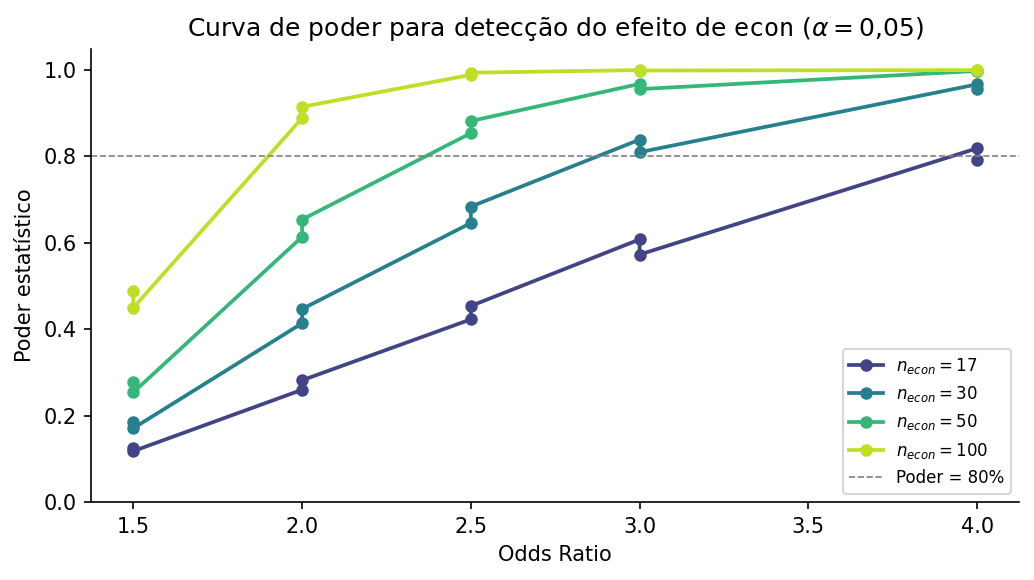
\includegraphics[width=0.80\textwidth]{analise/outputs/figures/forestplots/power_curve.png}
\nota{Linha vertical tracejada em OR $= 2{,}0$: poder $= 28{,}2\%$. Para atingir 80\% de poder com OR $= 2{,}0$, seriam necessários $n_{\texttt{econ}} \geq 120$.}
\label{fig:power_curve_v2}
\end{figure}

% ----------------------------------------------------------
\chapter{Repositório de Códigos e Dados}
% ----------------------------------------------------------
\label{ap:repo}

\section*{URL e versão}
Repositório oficial: \url{https://github.com/Schadenlord/tcc_esag}

\section*{Conteúdo e reprodutibilidade}
O pipeline de análise v2 está em \texttt{analise/}, com ponto de entrada único em \texttt{run\_all.py}. Para reproduzir integralmente todas as tabelas e figuras:

\begin{verbatim}
cd analise
python3 run_all.py --fast
\end{verbatim}

O flag \texttt{--fast} utiliza cache quando disponível. Para reanálise completa a partir dos dados brutos:

\begin{verbatim}
python3 run_all.py --no-cache
\end{verbatim}

Todas as dependências estão documentadas em \texttt{requirements.txt} no repositório. A semente aleatória (\texttt{BOOTSTRAP\_SEED = 42}) é fixada globalmente em \texttt{config.py} para reprodutibilidade integral.

\section*{Ética e LGPD}
Os dados disponibilizados no repositório são agregados e, portanto, estritamente anonimizados, sem identificação direta, em conformidade com o Parecer Consubstanciado nº 7.719.326 do CEP/UDESC e com a LGPD. Dados brutos sensíveis não são publicados.

\end{apendicesenv}
